\documentclass[11pt]{article}
\usepackage[margin=1in]{geometry}
\usepackage{fontspec}
\usepackage{booktabs}
\usepackage{longtable}
\usepackage{array}
\usepackage{float}
\usepackage{graphicx}
\usepackage{adjustbox}
\usepackage[font=small,labelfont=bf]{caption}
\usepackage{natbib}
\usepackage{xurl}
\usepackage[hidelinks]{hyperref}
\usepackage{setspace}
\setstretch{1.15}
\graphicspath{{../figs/}}
% Generated by scripts/tables.R; do not edit.
\newcommand{\nAlumni}{339}
\newcommand{\nStaff}{173}
\newcommand{\nMturk}{1,059}
\newcommand{\cueAlumni}{$-$31}
\newcommand{\cueAlumniSe}{3}
\newcommand{\cueStaff}{$-$27}
\newcommand{\cueStaffSe}{4}
\newcommand{\cueMturk}{$-$9}
\newcommand{\cueMturkSe}{2}
\newcommand{\cueLenientAlumni}{$-$37}
\newcommand{\cueLenientStaff}{$-$37}
\newcommand{\cueLenientMturk}{$-$16}
\newcommand{\cueWrongAlumni}{18}
\newcommand{\cueWrongStaff}{13}
\newcommand{\cueWrongMturk}{3}
\newcommand{\cueDkAlumni}{19}
\newcommand{\cueDkStaff}{25}
\newcommand{\cueDkMturk}{13}
\newcommand{\sarkozyName}{74}
\newcommand{\sarkozyPhoto}{28}
\newcommand{\robertsName}{40}
\newcommand{\robertsPhoto}{18}
\newcommand{\partialAlumni}{14}
\newcommand{\partialStaff}{13}
\newcommand{\partialMturk}{13}
\newcommand{\formAlumni}{5}
\newcommand{\formAlumniSe}{4}
\newcommand{\formStaff}{7}
\newcommand{\formStaffSe}{5}
\newcommand{\formCorrAlumni}{$-$1}
\newcommand{\formCorrStaff}{0}
\newcommand{\dkCorrectAlumni}{4}
\newcommand{\dkCorrectAlumniSe}{3}
\newcommand{\dkCorrectStaff}{$-$1}
\newcommand{\dkCorrectStaffSe}{4}
\newcommand{\dkDkAlumni}{$-$4}
\newcommand{\dkDkStaff}{$-$2}
\newcommand{\probeGainMax}{16}
\newcommand{\probeGainMin}{1}
\newcommand{\probeMturkMin}{17}
\newcommand{\probeMturkMax}{31}
\newcommand{\gapPanel}{18}
\newcommand{\gapMturkPolicy}{22}
\newcommand{\travelMc}{78}
\newcommand{\travelCertain}{60}
\newcommand{\travelKnown}{27}
\newcommand{\heardBush}{73}
\newcommand{\heardAca}{47}
\newcommand{\heardBan}{91}
\newcommand{\heardBushWrong}{32}
\newcommand{\inferAca}{37}
\newcommand{\guessAca}{14}
\newcommand{\lookedBush}{2}
\newcommand{\nItems}{102}
\newcommand{\nItemsTwelve}{59}
\newcommand{\nItemsSixteen}{43}
\newcommand{\featProbe}{9}
\newcommand{\featOpen}{13}
\newcommand{\featOpinion}{13}
\newcommand{\featSeven}{45}
\newcommand{\featSelfFilter}{43}
\newcommand{\anesGainMax}{13}
\newcommand{\anesGainMin}{0}
\newcommand{\naesGainMax}{1}
\newcommand{\anesConvertMax}{35}
\newcommand{\anesConvertMedian}{6}
\newcommand{\naesConvertMax}{2}


\title{Mis-measuring Political Knowledge? Do People Know More---or Even Less---about Politics than Commonly Thought?}
\author{Robert C. Luskin \and Gaurav Sood \and Daniel Weitzel}
\date{}

\begin{document}
\maketitle

\begin{abstract}
\noindent It has long been accepted that the public knows little about politics, but a number of revisionist studies claim that it knows appreciably more than conventional measures show: incorrect and ``don't know'' (DK) responses may conceal knowledge, questions may miss what people know, and coding may treat partially correct answers as wrong. This accounting neglects the other side of the ledger. Correct responses may be lucky guesses, shrewd inferences, or mere suspicion; questions may be too easy; and respondents may know more than the public from which they are drawn. We weigh both sides, adding randomized experiments in three online surveys (\nAlumni{} university alumni and \nStaff{} staff in 2010, \nMturk{} Mechanical Turk workers in 2017) and a recount of the design of the \nItems{} knowledge items in the 2012 and 2016 American National Election Studies. The hidden knowledge the revisionists point to is small. Asking people to identify officials from photos rather than names lowers correct identification, by \cueAlumni{} to \cueMturk{} percentage points. Multiple-choice versions of open-ended items and multiple-choice probes of open-ended nonanswers add little once guessing is accounted for, and discouraging DKs changes little. Measures that ask for confidence rather than a choice find much less knowledge than multiple-choice items do. On balance, conventional measures more likely overstate than understate what people know.
\end{abstract}

\section{Introduction}

Conventional survey measurements suggest that most people know relatively little about politics \citep{dellicarpini1996, luskin1987, kinder1998, price1999}. It is hard to quantify this impression very precisely, but the modal view is in the ballpark of the 40--45\% of respondents answering correctly the items assembled by \citet{dellicarpini1996} and by \citet{jerit2012} and \citet{barabas2014}. These percentages may not seem that low, but they come mostly from easy, closed-ended items with two, three, or four response options. If everyone guessed blindly, knowing nothing at all, 25--50\% would answer correctly by chance. Evidence of this sort is why the ``Panglossian impulse'' \citep{luskin2002} largely retreated from ``denial'' to ``extenuation,'' conceding that most people do not know much about politics but arguing that their attitudes and votes are not much affected \citep{lupia1994, popkin1991}.

Over the past couple of decades, however, some prominent revisionist studies have been walking back this concession, arguing that conventional measures significantly understate the public's knowledge. The questions, they claim, do too little to embolden the timid and engage the apathetic, who may say they don't know when in fact they do \citep{mondak2001, prior2008}; may miss fugitive knowledge, which respondents have but cannot recall in the moment \citep{prior2008}; may generate partially correct responses that are scored as incorrect \citep{gibson2009, debell2013}; and, being textual, may miss visual knowledge \citep{prior2014}. They may also ask about information too inconspicuous or unimportant to be noticed or readily recalled \citep{lupia2016, boudreau2011}.

There may be something to these claims, but they are one side of the ledger. Most knowledge questions are closed-ended, yielding correct responses that may be lucky guesses or shrewd inferences rather than knowledge \citep{luskin2002, luskin2011, bullock2015, prior2015}. Most do little to discourage guessing \citep{luskin2011, cor2016}, and some actively encourage it, by pressing respondents to guess, by posing the question as one of opinion rather than fact, or by supplying background information. Respondents may learn from earlier portions of the questionnaire. In online surveys, they may look answers up \citep{clifford2016}. And respondents may simply be more knowledgeable than the population from which they are drawn \citep{krupnikov2014}.

We weigh these upward and downward biases, drawing on the existing evidence and adding four kinds of new evidence. First, we recount the design features of every knowledge item in the 2012 and 2016 American National Election Studies (ANES). Second, we revisit the DK probes the ANES and the National Annenberg Election Study (NAES) fielded in 2000--2008. Third and fourth, we report randomized experiments in three online surveys: of alumni (\nAlumni{}) and staff (\nStaff{}) of a large private university in the western U.S., both in the fall of 2010, and of \nMturk{} U.S. workers on Amazon's Mechanical Turk (MTurk) in March 2017. None of the three is a probability sample of the public; we use them for what randomization within them licenses, comparisons of question designs.

The short of it is that the knowledge the revisionists say conventional measures miss is hard to find. Photos lower correct identification of public figures rather than raising it. Offering the answer in a menu, after an open-ended question or instead of one, adds few correct answers beyond what guessing would produce. Discouraging DKs changes little. By contrast, asking respondents how sure they are rather than which option is right shrinks the share who can be said to know the answer, often by half or more.

\section{Political Knowledge}

What is ``political knowledge''? Deeper questions about what it means to know something aside, knowledge is a matter of stored cognition---of mental representations of the phenomenal world. These include simple perceptions of objects and attributes but also, relevantly for politics, higher-order cognitions linking objects and attributes, expressible as sentences. Not all stored cognition is knowledge. Some is mere belief, less confidently held. To count as knowledge, a cognition must be both confidently held and correct, roughly the traditional philosophical understanding of knowledge as justified true belief \citep{sosa1991}. Misinformation, by contrast, is confidently held, incorrect belief, and mere belief may be correct or incorrect. Here we are concerned to distinguish knowledge from everything else, leaving the separation of misinformation from ignorance to a companion paper \citep{luskin2018}.

Aggregating from cognitions to the people holding them, an individual's knowledge of a domain is the share of the domain's elements that he or she knows \citep{luskin2026}. For political knowledge, the domain is everything political or politically relevant, a finite but ineffably large number of things, some of which no one need know. We need not be able to count them; this is the conceptual variable measures aim at.

Several points about knowledge in this sense need highlighting. First, it is a matter of ``how much,'' not ``what.'' The thrust of what someone knows matters for attitudes and votes, but so does the quantity, which figures to affect engagement and turnout and to condition other influences. Second, the universe of knowable, politically relevant information is vast and varied: institutions, constitutional and statutory provisions, policies, policy-relevant facts, the traits and records of officeholders, and the positions of candidates and parties. Some elements are more salient (more readily encountered), catchier (more readily retained), or more important (more capable of rationally changing other beliefs and attitudes) than others. Third, knowledge is a matter of existing, pre-measurement cognition. Questionnaires are reactive instruments that occasion as well as measure cognition \citep{webb1966}. Respondents pick up stray information and make inferences as they go, and what they learn or infer during an interview is not what they knew before it. Fourth, knowledge is not mere belief. Suspecting that something true is true is not knowing it. Fifth, ``partial knowledge'' means knowing some but not all of the relevant information \citep{luskin2011}; it comes into play in coding open-ended responses.

\section{Conventional Measurement}

Conventional measures score the share of a questionnaire's knowledge items a respondent answers correctly---``observed'' knowledge, in the terms of \citet{luskin2026}. This differs from knowledge as just defined in both numerator and denominator. The denominator is a small and highly nonrandom sliver of all that is knowable. The numerator counts items answered correctly, not items known.

The details vary from measure to measure but resemble each other enough to justify speaking of conventional measurement. The questions must be easy enough for question writers to think of and know the answers to, and at least some must be easy enough for many respondents to know, lest variation across respondents be mainly noise from lucky and unlucky guessing. The item sample thus skews toward the most salient and catchiest elements of the domain. A few kinds of questions are hardy perennials: civics-book questions about institutional rules, like the length of a Senate term; open-ended questions about the offices held by prominent figures; questions about which party controls a chamber; closed-ended questions about policy-relevant facts; and placements of candidates and parties on policy and ideological scales.

Table~\ref{tab:features} counts the design features of the \nItems{} knowledge items in the 2012 and 2016 ANES time series (\nItemsTwelve{} and \nItemsSixteen{} items). An item counts as a knowledge item if it asks about a state of the world, not the respondent's view or forecast, and one answer is correct by a nameable source; the coding rules and the item-by-item record are in the replication materials. No item offers an explicit DK option. Only \featOpen\% are open-ended. The most common format, at \featSeven\%, is the seven-point scale on which respondents place candidates and parties; scored as ``correct'' when the placement falls on the right side of the midpoint, it is effectively a two-option item. About \featOpinion\% invite an opinion (``do you think,'' ``would you say''), and \featProbe\% instruct face-to-face interviewers to probe DKs for a best guess. An earlier version of this table, built from a spreadsheet with one row per item and survey mode, overstated the probes because some items were entered more than once. It also counted every placement item as carrying a DK-encouraging preamble. The ``haven't you thought much about this?'' preamble in fact attaches to the respondent's self-placement; the candidate and party placements that follow carry an instruction not to probe DKs and offer none. Counting the preamble anyway would raise the share to \featSelfFilter\%.

\begin{table}[htbp]
\centering
\caption{Design features of the knowledge items in the 2012 and 2016 ANES time series.}
\label{tab:features}
\adjustbox{max width=\linewidth}{\begin{tabular}{lrrr}
\toprule
Feature & Combined ($n=102$) & 2012 & 2016 \\
\midrule
Explicit DK option & 0 [0, 4] & 0 & 0 \\
Interviewer probes DKs & 9 [5, 16] & 7 & 12 \\
Opinion-inviting wording & 13 [8, 21] & 14 & 12 \\
\quad ``Do you think'' & 7 [3, 13] & 7 & 7 \\
\quad ``Would you say'' & 6 [3, 12] & 7 & 5 \\
\quad ``Personal opinion'' & 2 [1, 7] & 2 & 2 \\
2 options & 11 [6, 18] & 8 & 14 \\
3 options & 9 [5, 16] & 7 & 12 \\
4 options & 19 [12, 27] & 24 & 12 \\
5 options & 0 [0, 4] & 0 & 0 \\
7 options (placement scales) & 45 [36, 55] & 47 & 42 \\
11 options & 4 [2, 10] & 3 & 5 \\
Open-ended & 13 [8, 21] & 10 & 16 \\
DK-encouraging preamble & 0 [0, 4] & 0 & 0 \\
DK-discouraging preamble & 0 [0, 4] & 0 & 0 \\
\bottomrule
\end{tabular}
}
\begin{minipage}{0.9\linewidth}\footnotesize
\emph{Note}: Entries are the percentage of items with each feature; 95\% Wilson intervals for the combined column in brackets. The unit is the question, counted once even when asked in both the face-to-face and web modes. ``Opinion-inviting'' is any of ``do you think,'' ``would you say,'' and ``in your personal opinion.'' Option counts are what respondents saw; placement scales are counted as 7- or 11-option items.
\end{minipage}
\end{table}

Knowledge questions also tend to be asked late in the questionnaire and to encourage substantive answers---by offering no DK option, urging respondents to give their best guess, probing volunteered DKs, or posing questions of fact as questions of opinion. The samples share much too. Most studies claiming external validity rest on a few sources, the ANES and the General Social Survey foremost among them, now joined by the Cooperative Congressional Election Study, the NAES, Pew Research Center surveys, and others, increasingly fielded by telephone or online.

\section{Sources of Bias}

A measure's error for an individual is the difference between his or her observed and true knowledge; its bias is the expected error, averaging across individuals and studies. The sources of bias are direct or indirect. The direct sources are respondent behavior, coding, item sampling, and unit sampling. The first three are matters of measurement; the fourth is a matter of whose knowledge is being measured. The indirect sources are question design and survey mode, which work through respondent behavior and, for mode, unit sampling as well.

Respondent behavior can err in six ways, three concealing knowledge and three veiling ignorance. \emph{Reticence}: respondents may say DK despite knowing, for fear of being wrong. \emph{Ennui}: they may be too bored to venture a substantive answer \citep{mondak2001, prior2008}. \emph{Failed retrieval}: they may blank on something they know, the ``tip-of-the-tongue'' phenomenon \citep{brown1966}. On the other side, \emph{guessing}: on closed-ended items, a blind pick is right one time in $k$ for $k$ options. \emph{Inference}: respondents who do not know an answer may reason their way to it, by eliminating options they know to be wrong or from stereotypes and side information. \emph{Cheating}: in self-administered online surveys, respondents may look answers up or ask someone \citep{clifford2016, vezzoni2017}.

The revisionist studies focus on the first three. How large are they? Probing initial DKs with something in the vein of ``give it a shot'' yields only a few more correct responses \citep{sturgis2008, luskin2011}. Paying a dollar for each correct answer raises the percentage correct by 3.6 points in the online experiment of \citet{prior2008}, and adding a day to recall, or to look up, the answers raises it by at most 5.6 points \citep[see also][]{bullock2015, prior2015}. Reticence, ennui, and failed retrieval together, in other words, do not seem to hide much. The sections below add new evidence on each, then turn to guessing, inference, and cheating.

\subsection{Probing Don't-Knows}

The most direct test of hidden knowledge is to ask again. Between 2000 and 2008, the ANES followed a DK to its open-ended office-recognition questions with ``Well, what's your best guess?'' and the NAES followed a DK to its questions about candidates' tax positions with ``Anyone come to mind?'' Neither probe offered options; each simply asked again. Table~\ref{tab:public} shows the results. On the ANES items, probing raised the share correct by \anesGainMin{} to \anesGainMax{} percentage points; on the NAES items, by at most \naesGainMax. Of the respondents probed, the median ANES item turned \anesConvertMedian\% into correct answers, the best (Dick Cheney in 2008) \anesConvertMax\%; no NAES item turned more than \naesConvertMax\%. Some of these conversions are themselves guesses. A respondent who offers ``vice president'' for Dick Cheney on being pressed may know it or may be choosing the likeliest office for a name he or she has heard often.

Our figures differ from those circulated in an earlier version of this paper in ways worth recording. The earlier DK columns counted only respondents who were probed, but interviewers often skipped the probe, so DKs were understated. The 2008 ANES answers were coded with keyword rules that credited ``Supreme Court justice'' as correct for John Roberts; we use the ANES's own codes and the same strict standard as in 2000 and 2004 \citep{krosnick2008}. Two NAES 2004 answer keys omitted candidates who held the keyed position, and one NAES 2008 item cannot be scored from the data we have. The 2000 ANES probe was meant to go to a random half of respondents, but a randomization failure put nearly everyone interviewed before November 16 on the unprobed form, so the 2000 comparison is within the probed form only.

\begin{table}[htbp]
\centering
\caption{Repeating the question after a don't-know: ANES and NAES, 2000--2008.}
\label{tab:public}
\adjustbox{max width=\linewidth}{\begin{tabular}{llrrrrrr}
\toprule
Survey & Item & $n$ & Before & After & Gain & DK before & DKs converted \\
\midrule
ANES 2000 & Trent Lott & 528 & 9 & 9 & 0.4 (0.3) & 67 & 1 \\
 & William Rehnquist & 528 & 12 & 12 & 0.4 (0.3) & 59 & 1 \\
 & Tony Blair & 529 & 33 & 36 & 2.5 (0.7) & 59 & 6 \\
 & Janet Reno & 529 & 52 & 56 & 3.6 (0.8) & 33 & 15 \\
ANES 2004 & Dennis Hastert & 1,066 & 10 & 11 & 1.2 (0.3) & 86 & 2 \\
 & Dick Cheney & 1,066 & 83 & 86 & 2.9 (0.5) & 14 & 28 \\
 & Tony Blair & 1,066 & 61 & 65 & 3.8 (0.6) & 32 & 18 \\
 & William Rehnquist & 1,066 & 29 & 31 & 1.7 (0.4) & 56 & 5 \\
ANES 2008 & Nancy Pelosi & 2,102 & 27 & 34 & 6.9 (0.6) & 65 & 11 \\
 & Dick Cheney & 2,102 & 54 & 67 & 12.8 (0.7) & 40 & 35 \\
 & Gordon Brown & 2,102 & 4 & 6 & 1.6 (0.3) & 86 & 2 \\
 & John Roberts & 2,102 & 4 & 5 & 0.9 (0.2) & 77 & 1 \\
NAES 2004 & Who favors making the tax cuts permanent & 21,141 & 65 & 65 & 0.3 (0.0) & 10 & 2 \\
 & Income above which Kerry would repeal the cuts & 31,940 & 33 & 34 & 0.4 (0.0) & 25 & 2 \\
 & Who would repeal the cuts for the wealthy & 2,151 & 49 & 49 & 0.8 (0.2) & 34 & 2 \\
 & Who would repeal all the cuts & 2,061 & 23 & 23 & 0.6 (0.2) & 44 & 1 \\
NAES 2008 & Republican who opposed the cuts (4 names) & 5,200 & 30 & 31 & 0.7 (0.1) & 38 & 2 \\
 & Republican who opposed the cuts (2 names) & 6,824 & 32 & 32 & 0.5 (0.1) & 25 & 2 \\
 & Democrat who would end cuts above an income & 20,895 & 41 & 41 & 0.2 (0.0) & 17 & 1 \\
 & Candidate who would end cuts above an income & 28,325 & 65 & 65 & 0.2 (0.0) & 13 & 2 \\
 & Democrat promising a working-family tax cut & 14,150 & 19 & 20 & 0.7 (0.1) & 34 & 2 \\
\bottomrule
\end{tabular}
}
\begin{minipage}{0.95\linewidth}\footnotesize
\emph{Note}: Percentages of respondents asked each item. ``Before'' is correct without probing, ``after'' correct with it; ``gain'' is the difference in percentage points, with standard errors in parentheses. ``DK before'' is the share giving no substantive first answer; ``DKs converted'' is the share of probed respondents whose second answer was correct. ANES office codes are the ANES's; the 2008 codes follow \citet{krosnick2008}. NAES keys are documented in the replication materials. Unweighted. The NAES microdata may not be redistributed; the replication materials include the item-level summaries.
\end{minipage}
\end{table}

In our 2010 surveys, respondents who left the open-ended question about Angela Merkel's or Mitch McConnell's office blank were then shown the same question as multiple choice with four offices and a DK option. In the 2017 MTurk survey, a random half of respondents answered a four-option multiple-choice version of the Merkel and McConnell questions right after the open-ended block, whatever they had answered. Table~\ref{tab:probes} shows how many respondents who had not answered the open-ended question correctly then chose the right office, before and after subtracting the right answers that guessing alone would produce. A respondent choosing at random among four options is wrong three times for each time he or she is right, so we count each wrong choice as implying a third of a lucky right one.

In 2010, the guessing-corrected gain ranges from \probeGainMin{} to \probeGainMax{} percentage points of the whole sample. It is largest for the photo version of the Merkel question, where many respondents had failed to recognize her. It is larger in 2017, \probeMturkMin{} to \probeMturkMax{} points. But the 2017 design differs in ways that inflate the gain: everyone in the multiple-choice arm saw the menu, including those who had given a partial or wrong answer; the menu followed the open-ended question within minutes, inviting respondents to reconsider; and online, unsupervised respondents could look the answers up. Recognizing the right office in a lineup after being asked about it moments before is some evidence of knowledge, but weaker evidence than naming it.

\begin{table}[htbp]
\centering
\caption{Multiple-choice follow-ups to open-ended identification questions.}
\label{tab:probes}
\adjustbox{max width=\linewidth}{\begin{tabular}{lllrrrrrr}
\toprule
Sample & Figure & Cue & $n$ & Open & Asked MC & Gain & Corr. gain & Open + corr. \\
\midrule
Alumni, 2010 & Angela Merkel & name & 184 & 64 & 14 & 6 (2) & 6 (2) & 70 \\
 &  & photo & 155 & 32 & 30 & 16 (3) & 16 (3) & 48 \\
 & Mitch McConnell & name & 184 & 31 & 29 & 2 (1) & 1 (1) & 32 \\
 &  & photo & 155 & 8 & 45 & 6 (2) & 6 (2) & 13 \\
Staff, 2010 & Angela Merkel & name & 93 & 43 & 28 & 9 (3) & 7 (3) & 50 \\
 &  & photo & 80 & 16 & 42 & 16 (4) & 15 (4) & 32 \\
 & Mitch McConnell & name & 93 & 13 & 32 & 4 (2) & 3 (2) & 15 \\
 &  & photo & 80 & 8 & 51 & 5 (2) & 3 (3) & 10 \\
MTurk, 2017 & Angela Merkel & name & 270 & 48 & 52 & 19 (2) & 17 (2) & 65 \\
 &  & photo & 284 & 44 & 56 & 25 (3) & 23 (3) & 68 \\
 & Mitch McConnell & name & 270 & 23 & 77 & 33 (3) & 31 (3) & 54 \\
 &  & photo & 284 & 26 & 74 & 30 (3) & 27 (3) & 54 \\
\bottomrule
\end{tabular}
}
\begin{minipage}{0.95\linewidth}\footnotesize
\emph{Note}: Percentages of all respondents assigned to each cue. ``Open'' is the share naming the office correctly. ``Asked MC'' is the share who did not name it correctly and were shown the multiple-choice version: in 2010, those who left the open-ended item blank; in 2017, everyone in the multiple-choice arm. ``Gain'' is the share who then chose the right office; ``corr.\ gain'' subtracts a third of the share choosing a wrong office. Standard errors in parentheses. ``Open + corr.'' adds the two.
\end{minipage}
\end{table}

\subsection{Open-Ended versus Multiple Choice}

A second test compares the same question asked open-ended and as multiple choice. Someone who knows the answer but cannot retrieve it should recognize it in a list. In the 2010 surveys, respondents were randomly asked either open-ended or multiple-choice versions of two general-knowledge questions: which country suffered the most casualties in World War II (the Soviet Union, of five listed countries) and the most common cause of death among American women (heart disease, of four causes). Table~\ref{tab:forms} shows the results. Pooling the two items, the multiple-choice versions produced \formAlumni{} (standard error \formAlumniSe) more percentage points of correct answers among alumni and \formStaff{} (\formStaffSe) among staff, neither distinguishable from zero. Correcting for guessing erases even that: \formCorrAlumni{} and \formCorrStaff{} points. Open-ended answers that named a hedge including the right answer (``Russia or Germany'') were counted correct, which if anything favors the open-ended version.

\begin{table}[htbp]
\centering
\caption{Correct answers to open-ended and multiple-choice versions of two questions.}
\label{tab:forms}
\adjustbox{max width=\linewidth}{\begin{tabular}{llrrrrr}
\toprule
Sample & Item & Open & MC & MC corr. & MC $-$ open & Corr. $-$ open \\
\midrule
Alumni, 2010 & Most World War II casualties & 58 & 58 & 53 & 0 (5) & $-$5 (6) \\
 & Leading cause of death, U.S. women & 58 & 68 & 61 & 10 (5) & 3 (6) \\
 & Pooled & -- & -- & -- & 5 (4) & $-$1 (4) \\
Staff, 2010 & Most World War II casualties & 43 & 44 & 35 & 1 (8) & $-$8 (8) \\
 & Leading cause of death, U.S. women & 62 & 75 & 70 & 13 (7) & 7 (8) \\
 & Pooled & -- & -- & -- & 7 (5) & 0 (6) \\
\bottomrule
\end{tabular}
}
\begin{minipage}{0.95\linewidth}\footnotesize
\emph{Note}: Percentages correct. Respondents were randomly assigned to the open-ended or the multiple-choice (MC) version. ``MC corr.'' subtracts from the share correct the share wrong divided by the number of wrong options (four for World War II, three for cause of death). Differences in percentage points with standard errors in parentheses; pooled rows regress correctness on the version with item fixed effects and cluster standard errors by respondent.
\end{minipage}
\end{table}

\subsection{Discouraging Don't-Knows}

A third approach discourages DKs, urging respondents to think harder and to answer even when unsure \citep{mondak1999, mondak2001}. Discouraging DKs may coax out knowledge the timid would otherwise withhold, but it also produces more guessing and on-the-spot inference \citep{luskin2011, sturgis2008}. \citet{luskin2011} find that discouraging DKs ``does nearly twice as much harm (5.7\%) as good (2.8\%).''

In the 2010 surveys, respondents were randomly given one of two introductions to three questions about the federal budget deficit under Reagan (1981--88, increased), Clinton (1993--2000, decreased), and George W.\ Bush (2001--08, increased). One told respondents that if they could not think of the answer, they should not worry and should mark ``couldn't say''; the other asked them to give their best guess. Both offered ``couldn't say.'' A fourth question, about the deficit ``between 2009 and 2010, when Barack Obama was the president,'' was keyed ``increased,'' but the deficit fell, from \$1.41 trillion in fiscal 2009 to \$1.29 trillion in fiscal 2010 \citep{omb2026}, so we do not score it.

Table~\ref{tab:dk} shows that DKs were rare under either introduction, which left little room for discouragement to work. Pooling the three items, discouraging DKs lowered them by \dkDkAlumni{} points among alumni and \dkDkStaff{} among staff and changed the share correct by \dkCorrectAlumni{} (\dkCorrectAlumniSe) and \dkCorrectStaff{} (\dkCorrectStaffSe) points. Only for Reagan among alumni did discouragement raise the share correct appreciably.

\begin{table}[htbp]
\centering
\caption{DK-encouraging and DK-discouraging introductions to the deficit questions.}
\label{tab:dk}
\adjustbox{max width=\linewidth}{\begin{tabular}{llrrrrrrr}
\toprule
Sample & Deficit under & \multicolumn{2}{c}{Correct} & \multicolumn{2}{c}{DK} & \multicolumn{3}{c}{Discouraging $-$ encouraging}\\ & & Enc. & Disc. & Enc. & Disc. & Correct & DK & Corr. \\
\midrule
Alumni, 2010 & Reagan, 1981--88 & 62 & 74 & 15 & 5 & 12 (5) & $-$10 (3) & 13 (7) \\
 & Clinton, 1993--2000 & 79 & 76 & 4 & 3 & $-$3 (5) & $-$1 (2) & $-$5 (7) \\
 & G. W. Bush, 2001--08 & 93 & 96 & 1 & 1 & 2 (3) & 0 (1) & 3 (4) \\
 & Pooled & -- & -- & -- & -- & 4 (3) & $-$4 (2) & 4 (4) \\
Staff, 2010 & Reagan, 1981--88 & 68 & 66 & 10 & 8 & $-$1 (7) & $-$2 (4) & $-$3 (10) \\
 & Clinton, 1993--2000 & 81 & 78 & 4 & 1 & $-$3 (6) & $-$3 (2) & $-$6 (9) \\
 & G. W. Bush, 2001--08 & 95 & 95 & 3 & 1 & 0 (3) & $-$2 (2) & 0 (4) \\
 & Pooled & -- & -- & -- & -- & $-$1 (4) & $-$2 (2) & $-$3 (5) \\
\bottomrule
\end{tabular}
}
\begin{minipage}{0.95\linewidth}\footnotesize
\emph{Note}: Percentages correct and DK, by randomly assigned introduction. ``Corr.'' is the share correct minus half the share wrong (two wrong options). Differences in percentage points with standard errors in parentheses; pooled rows as in Table~\ref{tab:forms}.
\end{minipage}
\end{table}

\subsection{Guessing, Inference, and Mere Belief}

Blind guessing is hard, and therefore rare, on open-ended items. On closed-ended items it takes only a pick. The standard correction for guessing treats every wrong answer as evidence of a blind guess and subtracts the lucky right answers that many guesses imply. But that correction assumes that everyone who does not know guesses at random, and it cannot touch correct answers that come from inference or mere suspicion. A different design asks respondents not to choose but to say how sure they are that each option is right. Knowing then means being certain of the right option and surer of it than of any wrong one.

We randomly assigned respondents to multiple-choice items or to confidence ratings of the same options: in 2010, for the photos of Robert Gates and Stephen Breyer and two provisions of the Affordable Care Act; in 2017, for the same two provisions, the 2017 executive order on travel from several majority-Muslim countries, and Merkel's and McConnell's offices. Figure~\ref{fig:formats} and Table~\ref{tab:formats} show that multiple-choice items credit far more respondents with knowing the answer than confidence ratings do, even after the guessing correction. Averaging across items, the corrected multiple-choice share exceeds the confident share by \gapPanel{} points in the 2010 surveys and by \gapMturkPolicy{} points on the 2017 policy items. On the travel ban, \travelMc\% chose the right answer from the menu and \travelCertain\% were certain it was right, but only \travelKnown\% were certain of it and less sure of every wrong answer; many were equally sure that the order stripped green cards from immigrants. The gap is smallest for the office questions asked by name, which followed an open-ended question about the same person. A companion paper applies the same comparison to misinformation \citep{luskin2018}.

\begin{figure}[htbp]
\centering
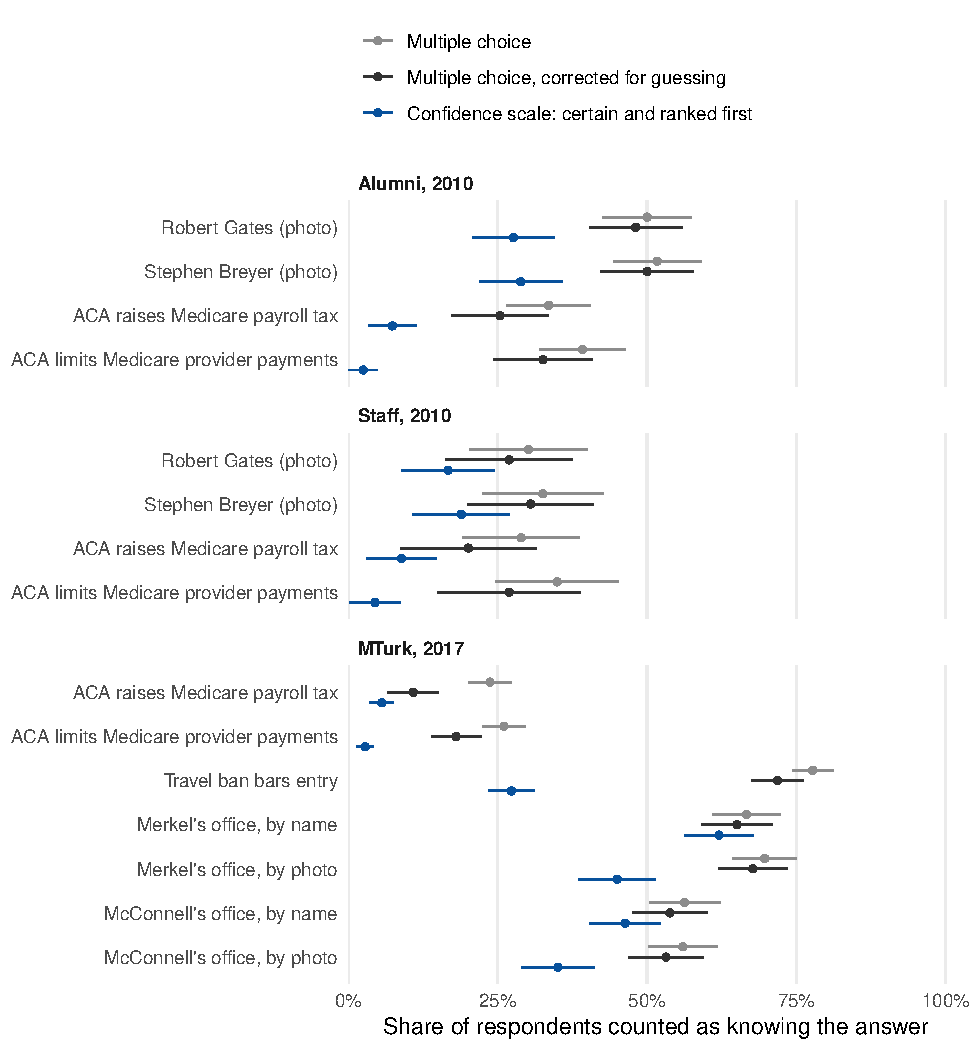
\includegraphics[width=\linewidth]{formats}
\caption{Share of respondents counted as knowing the answer, by format. Respondents were randomly assigned to multiple choice or to rating how sure they were of each option (0--10 in 2010 and on the 2017 policy items, 0--100 on the 2017 office items). On the scale, knowing means rating the right option at the top of the scale and above every wrong option. The guessing correction subtracts a third of the share choosing a wrong option. Bars are 95\% intervals.}
\label{fig:formats}
\end{figure}

\begin{table}[htbp]
\centering
\caption{Knowledge by multiple choice and by confidence rating.}
\label{tab:formats}
\adjustbox{max width=\linewidth}{\begin{tabular}{llrrrrr}
\toprule
Sample & Item & MC & MC corr. & Certain & Certain, first & MC corr. $-$ scale \\
\midrule
Alumni, 2010 & Robert Gates (photo) & 50 & 48 & 28 & 28 & 20 (5) \\
 & Stephen Breyer (photo) & 52 & 50 & 29 & 29 & 21 (5) \\
 & ACA raises Medicare payroll tax & 34 & 25 & 12 & 7 & 18 (5) \\
 & ACA limits Medicare provider payments & 39 & 33 & 5 & 2 & 30 (4) \\
Staff, 2010 & Robert Gates (photo) & 30 & 27 & 17 & 17 & 10 (7) \\
 & Stephen Breyer (photo) & 33 & 31 & 19 & 19 & 12 (7) \\
 & ACA raises Medicare payroll tax & 29 & 20 & 11 & 9 & 11 (7) \\
 & ACA limits Medicare provider payments & 35 & 27 & 9 & 4 & 22 (6) \\
MTurk, 2017 & ACA raises Medicare payroll tax & 24 & 11 & 10 & 6 & 5 (2) \\
 & ACA limits Medicare provider payments & 26 & 18 & 4 & 3 & 15 (2) \\
 & Travel ban bars entry & 78 & 72 & 60 & 27 & 45 (3) \\
 & Merkel's office, by name & 67 & 65 & 64 & 62 & 3 (4) \\
 & Merkel's office, by photo & 70 & 68 & 46 & 45 & 23 (4) \\
 & McConnell's office, by name & 56 & 54 & 47 & 46 & 7 (4) \\
 & McConnell's office, by photo & 56 & 53 & 35 & 35 & 18 (4) \\
\bottomrule
\end{tabular}
}
\begin{minipage}{0.95\linewidth}\footnotesize
\emph{Note}: Percentages of each randomly assigned arm. MC: chose the right option. MC corr.: minus a third of the share choosing a wrong one. Certain: rated the right option at the top of the scale. Certain, first: did so and rated every wrong option lower. The last column is MC corr.\ minus certain, first, in percentage points, with standard errors in parentheses.
\end{minipage}
\end{table}

What lies behind correct multiple-choice answers? In the 2017 survey, a random two-thirds of respondents were asked, after several multiple-choice items, what made them choose their answer, from a list: they had read, seen, or heard it; it made sense in view of other things they knew; they took a shot; it felt good to think it; they asked someone; or they looked it up. Table~\ref{tab:reasons} shows the reasons given for correct and incorrect answers. Where the fact is widely reported---the travel ban---\heardBan\% of those answering correctly said they had read or heard it. Where it is obscure---that the Affordable Care Act limits increases in payments to Medicare providers---only \heardAca\% did; \inferAca\% said they inferred the answer and \guessAca\% that they guessed. Self-reports understate guessing, which respondents have reason to be shy about, and cheating, which they have more reason still to hide; only \lookedBush\% of those answering the Bush deficit question correctly admitted to asking someone or looking it up. Even taken at face value, a sizable share of correct answers to less-publicized facts come from inference or luck. Incorrect answers, notably, are also mostly attributed to something heard: \heardBushWrong\% of those who said the deficit did not rise under Bush said so.

\begin{table}[htbp]
\centering
\caption{Reasons given for multiple-choice answers, 2017 MTurk survey.}
\label{tab:reasons}
\adjustbox{max width=\linewidth}{\begin{tabular}{llrrrrrrr}
\toprule
Item & Answer & $n$ & Heard it & Inferred & Guessed & Felt good & Asked & Looked up \\
\midrule
Deficit rose under G. W. Bush & correct & 508 & 73 & 19 & 5 & 0 & 0 & 2 \\
 & incorrect & 66 & 32 & 23 & 29 & 6 & 3 & 8 \\
ACA limits Medicare provider payments & correct & 94 & 47 & 37 & 14 & 2 & 0 & 0 \\
 & incorrect & 96 & 48 & 29 & 21 & 2 & 0 & 0 \\
Travel ban bars entry & correct & 284 & 91 & 6 & 1 & 0 & 0 & 1 \\
 & incorrect & 77 & 62 & 23 & 9 & 3 & 0 & 3 \\
\bottomrule
\end{tabular}
}
\begin{minipage}{0.95\linewidth}\footnotesize
\emph{Note}: Percentages of substantive answers giving each reason, among respondents randomly assigned to the closed reason probe (and, for the two policy items, to multiple choice). The Obama deficit item is not scored (see text).
\end{minipage}
\end{table}

\subsection{Names versus Photos}

The conventional open-ended items ask respondents to identify political figures by name. It has been argued that more people recognize faces than names. Images are more easily encoded, stored, and recalled than words \citep{grimes1991, lang1995, lang1999}, television is a heavily visual medium, and \citet{prior2014} finds that asking about photos rather than names can yield more correct answers.

Our surveys randomly asked respondents to identify public figures either by name or from a photo, open-ended, with the same instructions. Figure~\ref{fig:cue} and Table~\ref{tab:cue} show that photos made correct identification less likely, not more. Pooling figures, the share naming the office correctly fell by \cueAlumni{} (standard error \cueAlumniSe) percentage points among alumni, \cueStaff{} (\cueStaffSe) among staff, and \cueMturk{} (\cueMturkSe) on MTurk. \sarkozyName\% of alumni identified Nicolas Sarkozy as president of France from his name; \sarkozyPhoto\% did from his photo. Photos also produced more wrong answers (by \cueWrongAlumni, \cueWrongStaff, and \cueWrongMturk{} points) and more blanks (\cueDkAlumni, \cueDkStaff, and \cueDkMturk{} points). Many of the wrong answers were confident misidentifications of someone else in the news: Sarkozy's photo as the White House chief of staff, Janet Napolitano's as the newest Supreme Court justice, and Merkel's as the governor of Arizona or a candidate for office.

The contrast with \citet{prior2014} probably lies in format. His visual items offered response options; ours asked respondents to supply the office, as the conventional name items do. \citet{munzert2017}, who also asked about leaders' offices open-ended in an experiment in the German Longitudinal Election Study, find that visual and verbal items form equally strong knowledge scales. A face may be enough to recognize the right answer in a lineup without being enough to recall it. Whatever the reason, open-ended photo items do not uncover knowledge that name items miss. Note too that the question applies only to items about people. Much consequential political knowledge, of policy-relevant facts for instance, cannot be asked about with photos.

\begin{figure}[htbp]
\centering
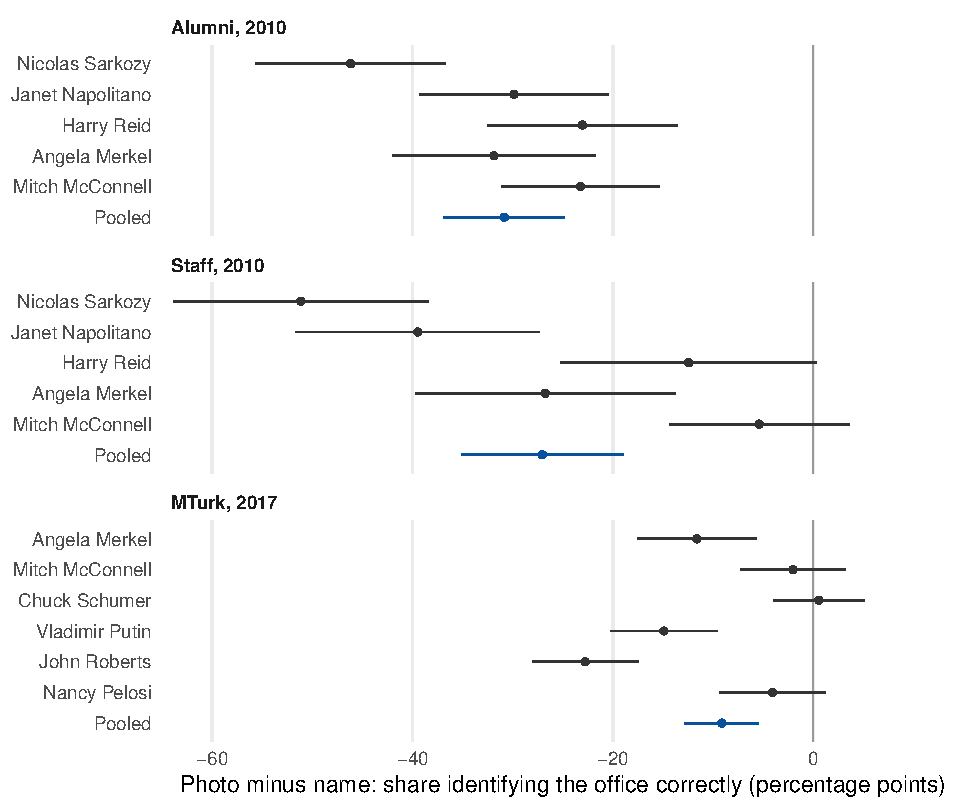
\includegraphics[width=\linewidth]{cue}
\caption{Difference in the share identifying a public figure's office correctly when asked by photo rather than by name, open-ended. Respondents were randomly assigned to one version. Pooled estimates regress correct identification on the photo arm with figure fixed effects, clustering by respondent. Bars are 95\% intervals.}
\label{fig:cue}
\end{figure}

\begin{table}[htbp]
\centering
\caption{Identifying public figures by name and by photo.}
\label{tab:cue}
\adjustbox{max width=\linewidth}{\begin{tabular}{llrrrr}
\toprule
Sample & Public figure & Name & Photo & Photo $-$ name & Lenient \\
\midrule
Alumni, 2010 & Nicolas Sarkozy & 74 & 28 & $-$46 (5) & $-$54 (5) \\
 & Janet Napolitano & 47 & 17 & $-$30 (5) & $-$39 (5) \\
 & Harry Reid & 42 & 19 & $-$23 (5) & $-$24 (5) \\
 & Angela Merkel & 64 & 32 & $-$32 (5) & $-$43 (5) \\
 & Mitch McConnell & 31 & 8 & $-$23 (4) & $-$26 (5) \\
 & Pooled & -- & -- & $-$31 (3) & $-$37 (3) \\
Staff, 2010 & Nicolas Sarkozy & 70 & 19 & $-$51 (6) & $-$51 (7) \\
 & Janet Napolitano & 49 & 10 & $-$39 (6) & $-$52 (6) \\
 & Harry Reid & 31 & 19 & $-$12 (7) & $-$27 (7) \\
 & Angela Merkel & 43 & 16 & $-$27 (7) & $-$36 (7) \\
 & Mitch McConnell & 13 & 8 & $-$5 (5) & $-$22 (6) \\
 & Pooled & -- & -- & $-$27 (4) & $-$37 (5) \\
MTurk, 2017 & Angela Merkel & 52 & 41 & $-$12 (3) & $-$15 (3) \\
 & Mitch McConnell & 26 & 24 & $-$2 (3) & $-$11 (3) \\
 & Chuck Schumer & 17 & 17 & 1 (2) & $-$11 (3) \\
 & Vladimir Putin & 80 & 65 & $-$15 (3) & $-$15 (2) \\
 & John Roberts & 40 & 18 & $-$23 (3) & $-$32 (3) \\
 & Nancy Pelosi & 28 & 24 & $-$4 (3) & $-$12 (3) \\
 & Pooled & -- & -- & $-$9 (2) & $-$16 (2) \\
\bottomrule
\end{tabular}
}
\begin{minipage}{0.95\linewidth}\footnotesize
\emph{Note}: Percentages naming the office correctly, by randomly assigned cue, and the photo-minus-name difference in percentage points with standard errors in parentheses. ``Lenient'' also counts partially correct answers, such as ``senator'' for a party leader in the Senate. Pooled rows as in Figure~\ref{fig:cue}.
\end{minipage}
\end{table}

\section{Coding}

Closed-ended items make one option correct and the others incorrect. Open-ended answers may be partially correct. ``Senator'' for Mitch McConnell contains real information but misses his being the Senate's Republican leader; ``politician'' contains a sliver, and perhaps only an inference from the questionnaire's being about politics. Coding such answers as incorrect understates knowledge, but coding them as correct would overstate it \citep{gibson2009, krosnick2008, debell2013}.

We coded every open-ended answer in our surveys with one set of rules, published with the replication materials along with every distinct answer and its code. Naming the office (``Senate majority leader,'' ``German chancellor,'' ``chief justice'') is correct, as are misspellings and hedges that include the right office. The right institution without the office (``senator,'' ``Supreme Court justice,'' ``German president'') is partially correct. Partially correct answers were \partialAlumni\% of all responses among alumni, \partialStaff\% among staff, and \partialMturk\% on MTurk. Counting them as correct would raise the share identifying each figure, but it would not change any comparison above: the lenient photo penalty in Table~\ref{tab:cue} is at least as large as the strict one.

Just as some answers coded incorrect contain elements of the right one, some coded correct miss elements or mix in errors. The binary coding of partially correct answers cuts both ways.

\section{Item Sampling}

Survey items could be harder or easier than the domain from which they are drawn. Some argue that knowledge items stray too far from the headlines or ask about information of too little use to ordinary citizens \citep{lupia2006, lupia2016, boudreau2011}. But the conventional batteries---which party controls Congress, where the parties stand, what offices prominent figures hold---can hardly be faulted for straying from the mainstream. Conventional measures correlate with turnout and interest and predict voting ``correctly'' \citep{lau1997} and in line with economic interests \citep{gomez2001}. Knowledge of disparate facts is highly correlated across large batteries \citep{dellicarpini1996, barabas2014}, which is why a few items can measure it reliably \citep{dellicarpini1993}. And behavioral data give little reason to think the public knows much that surveys miss: in browsing records from 1.2 million users of a web browser toolbar, \citet{flaxman2016} find that only about 4\% read at least ten substantive news articles and two opinion pieces over three months.

More plausibly, conventional measures overstate knowledge through item sampling. The domain of knowable political facts is vast, and even the best informed know a vanishingly small fraction of it \citep{luskin2026}. That the average respondent answers half or more of a conventional battery correctly reflects sampling from the easy, salient end of the domain.

\section{Unit Sampling}

Respondents may be more or less knowledgeable than the population from which they are drawn. All probability samples of the public suffer nonresponse, and the least educated, least affluent, and most socially marginal---all attributes associated with less political knowledge---are the most elusive. Samples therefore tend to know more than the populations they represent. Online panels may make matters worse. Panelists interested in politics may persist longer, taking many surveys may make them more interested, and many panelists have taken hundreds of surveys \citep{hillygus2014}, rehearsing the conventional knowledge items along the way. Taking many political surveys may teach people the answers to the conventional items without teaching them more about public affairs generally \citep{ahler2017}. Our own samples illustrate the point in the extreme: university alumni and staff, most with college or graduate degrees, and MTurk workers, who take many surveys.

\section{Discussion}

There is a pertinacious Panglossian strain in the study of mass politics. At first it was simply supposed that most people knew quite a lot about politics. Then, in the face of overwhelming evidence that few knew very much, the claim became that their ignorance made little difference, because most people managed to approximate their ``full-information'' votes and opinions anyway. Now, in the face of growing evidence of large individual and aggregate departures from full-information preferences, the claim has rotated back: people know a lot more than commonly thought.

The evidence here provides little comfort for that view. Asking for recognition in place of recall, probing nonanswers, and discouraging DKs add few correct answers beyond what guessing would produce, and photos subtract. The forces pushing the other way---guessing, inference, looking answers up, easy items, and knowledgeable samples---are harder to measure, but where we can measure them, as in the comparison of multiple-choice choices with confidence ratings, they are large. If conventional measures are biased, they more likely overstate than understate what the public knows.

The new evidence has limits. The 2010 and 2017 samples are not probability samples of the public; they support comparisons of question designs, not estimates of how much Americans know. Some experiments have small arms. And each design isolates one source of bias at a time. The balance of evidence, however, points one way.

\bibliographystyle{apsr}
\bibliography{references}

\appendix
\section{Survey Designs}

\paragraph{Alumni and staff, 2010.} Both surveys were fielded online between September 9 and October 15, 2010, to panels of alumni and of staff of a large private university in the western U.S. We keep panel members' first complete attempt; the survey team's test entries and partial completes are excluded, leaving \nAlumni{} alumni and \nStaff{} staff. Respondents were independently randomized to (1) the name or photo version of the public-figure questions, (2) open-ended or multiple-choice versions of the World War II and cause-of-death questions, (3) multiple-choice or 0--10 confidence versions of the Gates, Breyer, and Affordable Care Act questions, and (4) the DK-encouraging or DK-discouraging introduction to the deficit questions. The public-figure questions asked, ``What job or office does each of the following currently hold?'' (or ``\ldots does the person in the photo currently hold?''), with instructions to give a best guess or leave the space blank.

\paragraph{MTurk, 2017.} Fielded on Qualtrics on March 27, 2017, to U.S. workers, with \nMturk{} respondents randomized. Respondents were independently randomized to (1) name or photo versions of the public-figure questions (``Here's a list of names [set of photos]. For each, can you tell me what position that person holds? If you don't know, don't worry about it. Just leave the space blank''), which also set whether the follow-up office questions used names or photos; (2) multiple-choice or 0--100 confidence versions of those follow-up questions; (3) multiple-choice or 0--10 confidence versions of the policy questions; (4) a closed or open probe of the reasons for their answers (two-thirds closed); and (5) a request, at the start, to pledge not to look answers up (two-thirds asked). A second greenhouse-gas question, which a last-minute edit left with two correct options, is not scored. Neither is a first greenhouse-gas question (``are greenhouse gases \ldots\ a cause of rising sea levels'') whose distractors include damage to the ozone layer and respiratory problems, both true of some greenhouse gases \citep{ravishankara2009}.

\end{document}
